




\section{Experiment}
\label{cp6:experiment}



% \gcm{earlier in the chapter you should probably cite the ethics certificate number the work was conducted under}
% \art{should this go under the preface?}

% \gcm{The figure would be better as a summary rather than introducing the chapter.}

% \gcm{Are there research questions?}

% Figure~\ref{fig:tool-experiment-procedures} presents an experiment designed to evaluate how a semantic-based tool might assists a software developer perform a task.


We seek to evaluate how a semantic-based tool might assists a software developer perform a task.
We consider three questions:


\begin{enumerate}[label=RQ\arabic*]
    \item Does usage of a semantic-based tool help developers produce more correct solutions? 
    \item How useful is the text identified by a semantic-based tool, i.e., does the text automatically identified contains information that assists task completion? 
    \item How does the text automatically identified by our semantic-based tool compare to text 
    that humans perceive as relevant to a task?
\end{enumerate}

% solution more often than if they had not used the tool?

% 


To answer these questions, we designed an experiment where 24 participants with software development background each attempted a
\textit{control} and \textit{tool-assisted} task randomly drawn from a list of well-known Python programming tasks.
Participants are asked to write a solution for both of their assigned tasks
and we use the control task to collect what text a participant deems relevant to the task at hand.
In the tool-assisted task, we gather input on the usefulness of the text automatically identified and shown by our tool. 
This design, summarized in Figure~\ref{fig:tool-experiment-procedures} and detailed in the following subsections,  allow us to:






\begin{itemize}
    \item assess the correctness of the solutions for each tasks performed \textit{with} or \textit{without} tool support, thus addressing \textit{RQ1};
     
    \item discuss the usefulness of the text automatically identified  according to the feedback provided by the participants, which helps us answer \textit{RQ2}, and;

    \item compare manual and tool identified task-relevant text, which addresses \textit{RQ3} and helps us cross-examine~\cite{easterbrook2008} results from Chapter~\ref{ch:identifying}. 
\end{itemize}
 


\begin{figure}[h!]
\centering
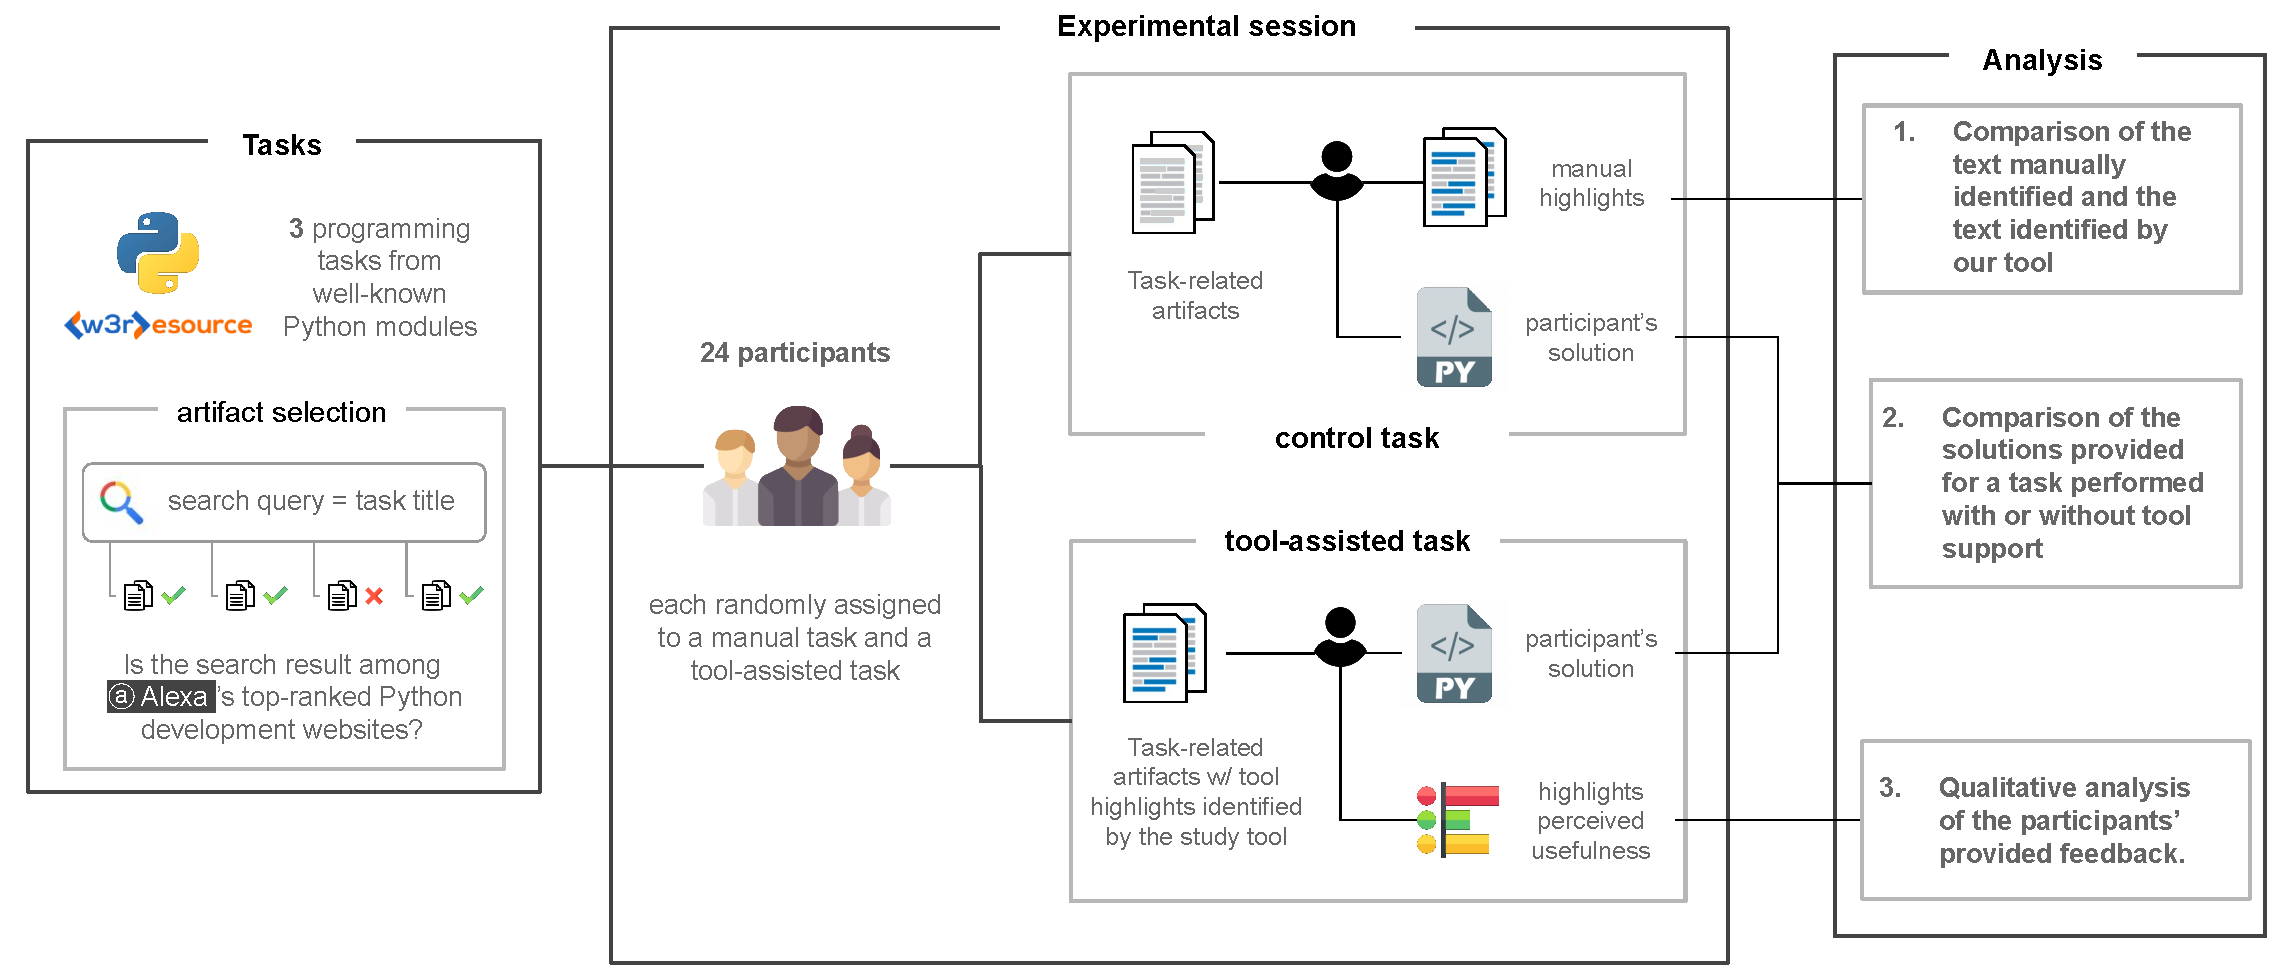
\includegraphics[width=1.0\textwidth]{cp6/tool-experiment-pipeline.pdf}
\caption{Summary of experimental procedures}
\label{fig:tool-experiment-procedures}
\end{figure}



The \acs{UBC} \acs{ERB} approved this experiment under the certificate \textit{H19-04054}.
The experiment's supplementary material is also publicly available~\cite{cp6_supplementary_material}.



\subsection{Tasks}
\label{cp6:tasks}


We opted for an experiment with tasks that could be completed by participants on their own time and computer.
This decision was motived by the COVID-19 pandemic and challenges related to recruiting participants and conducting an in-person experiment~\cite{russo2021a, russo2021b}. 
Since participants would follow instructions on their own, we decided to use tasks that are easy to understand and perform in a single experimental session, but that still required a participant  
to seek information in artifacts associated with each task.


Table~\ref{tbl:python-tasks-modules} details the tasks that we have selected based on task selection procedures from related work that meet these criteria~\cite{thiselton2019}. 
These tasks were drawn from
Python w3resource\footnote{\url{https://www.w3resource.com/python-exercises/}} tasks
that require usage of at least one module external to the Python core library.
By using external modules, we aim to reduce the likelihood that a participant 
can provide a solution for a task without consulting any of the artifacts (Section~\ref{cp6:experiment-artifacts})
that detail each of the modules associated with each task. 


Figure~\ref{fig:nytimes-task-github} provides an excerpt of the information shown in a task\footnote{Full descriptions are available in the experiment's supplementary material~\cite{cp6_supplementary_material}.}.
For each task, participants had the task description and examples of input and output scenarios at their disposal. A task contained a list of resources that participants could consult 
so that they could write their solution.
Each task also contained a link to an online coding environment (Section~\ref{cp6:coding-environment})
where a participant could write and test their solution. 









\subsection{Artifacts}
\label{cp6:experiment-artifacts}


% Note that our decision to control the artifacts shown per task relates to our need to study if there is overlap between the text that participants manually identify as relevant and the text that our semantic-based tool identifies for these same artifacts. 


Each task requires a set of artifacts that a participant could peruse for information that could assist them in writing their solution.
Ideally, participants could find these artifacts on their own. However, our need to compare solutions between participants who perform a task 
assisted by our tool and without it as well as our need to compare the text that participants deem relevant to the text
automatically identified by our tool means that all participants must have the exact same artifacts for a task.


Therefore,
we follow procedures similar to the ones we used to create the \acs{DS-android} dataset to produce the list of artifacts for each of the tasks in Table~\ref{tbl:python-tasks-modules}. 
That is, we use the Google search engine to obtain up to ten artifacts that likely contain 
information that could help a participant correctly complete that task. 
Three pilot runs ensured that the artifacts collected using such procedures had sufficient information to complete a task without 
the need of additional resources. Based on these pilots, we simplified the description of the \texttt{distances} tasks removing the need to sort the list suggested addresses, what also led to the removal of two artifacts associated with sorting. Table~\ref{tbl:python-task-distribution} details the kinds of artifacts per task.



\begin{table}
\centering
\caption{Python tasks}
\begin{footnotesize}
\rowcolors{2}{}{lightgray}
\begin{tabular}{ll}
\hline
\textbf{Task} & \textbf{Description}                                                                                         \\
\hline
\hline
%
\parbox[l][1cm][c]{1cm}{Practice task}       &
\parbox[l][1cm][c]{11cm}{Given three dictionaries representing address books,
you must write an algorithm using the Python core \texttt{dict} module to merge them.}    \\
\hline
%
Distances     &
\parbox[l][1.3cm][c]{11cm}{Given a string representing a rendezvou point and a list of suggested picnic addresses
    you must write an algorithm using the \texttt{geopy} module to find the  picnic address closest to the rendezvou point.} \\
%
NYTimes       &
\parbox[l][1cm][c]{11cm}{Given a string representing the url for NY Times Today's,
    write an algorithm using the \texttt{BeautifulSoup} and \texttt{requests} modules to scrape all the headlines of that page.}
\\
%
Titanic       &
\parbox[l][1cm][c]{11cm}{Given a string representing a url for the titanic dataset,
    you must write an algorithm using the \texttt{pandas} and \texttt{seaborn} modules to create a barchart of the data.}    \\
    
\hline
\end{tabular}
\end{footnotesize}
% \smallskip
\label{tbl:python-tasks-modules}
\end{table}





\subsection{Coding environment}
\label{cp6:coding-environment}



To ensure that participants had the same conditions to perform each task
and also to minimize setup instructions, we used Google Colab\footnote{\url{https://colab.research.google.com/}} as our coding environment. 
% \gcm{Say something here that Colab is an online coding notebook or something.}
Colab is a product from Goole Research that allows people to write and execute Python code through their browser~\cite{google-colab}. 
% The platform is well suited for 



Colab provided participants with a code editor with amenities commonly found in modern IDEs, e.g., code completion and syntax highlighting. It also ensured that all the participants 
performed the tasks in the same Python version and it lifted 
burdens that could arise from installing dependencies associated with the external modules used in each of our tasks. 


Figure~\ref{fig:nytimes-task-colab} shows an example of the Colab coding environment. 
First it handled dependencies management and then, 
it presented a class containing a single method with a \texttt{TODO} block where 
participants should write their solution. 
The environment also provided a main function where participants could see the output
of their code. Alternatively, a participant could use test cases to test their solution
against the examples shown in each task description.








\begin{table}
\centering
\caption{List of artifact types per task}
\begin{scriptsize}
\begin{threeparttable}
\rowcolors{2}{}{lightgray}
\begin{tabular}{llcllc}
\hline
\textbf{Task} & \textbf{Artifacts} & \textbf{Total} & \textbf{Task} & \textbf{Artifacts} & \textbf{Total}                                                                              \\
\hline
\hline
%
%
\parbox[l][0.5cm][c]{1cm}{Distances}    & API documents             & 2  & \parbox[l][0.5cm][c]{1cm}{NYTimes}      & API documents             & 3 \\
\parbox[l][0.5cm][c]{1cm}{}             & Stack Overflow posts      & 3 & \parbox[l][0.5cm][c]{1cm}{}             & Stack Overflow posts      & 3 \\
\parbox[l][0.5cm][c]{1cm}{}             & Miscellaneous web pages   & 3 & \parbox[l][0.5cm][c]{1cm}{}             & Miscellaneous web pages   & 4 \\
\hline

\parbox[l][0.5cm][c]{1cm}{Titanic}      & API documents             & 4 & \parbox[l][0.5cm][c]{1cm}{Practice\tnote{*}}      & API documents             & 1 \\
\parbox[l][0.5cm][c]{1cm}{}             & Stack Overflow posts      & 3 & \parbox[l][0.5cm][c]{1cm}{}             & Stack Overflow posts      & 2 \\
\parbox[l][0.5cm][c]{1cm}{}             & Miscellaneous web pages   & 3 \\
\hline


\end{tabular}
\begin{tablenotes}
    \item[*] smaller number of artifacts due to it being a practice task;
\end{tablenotes}
\end{threeparttable}
\end{scriptsize}
\label{tbl:python-task-distribution}
\end{table}










\clearpage

\begin{figure}
    \centering
    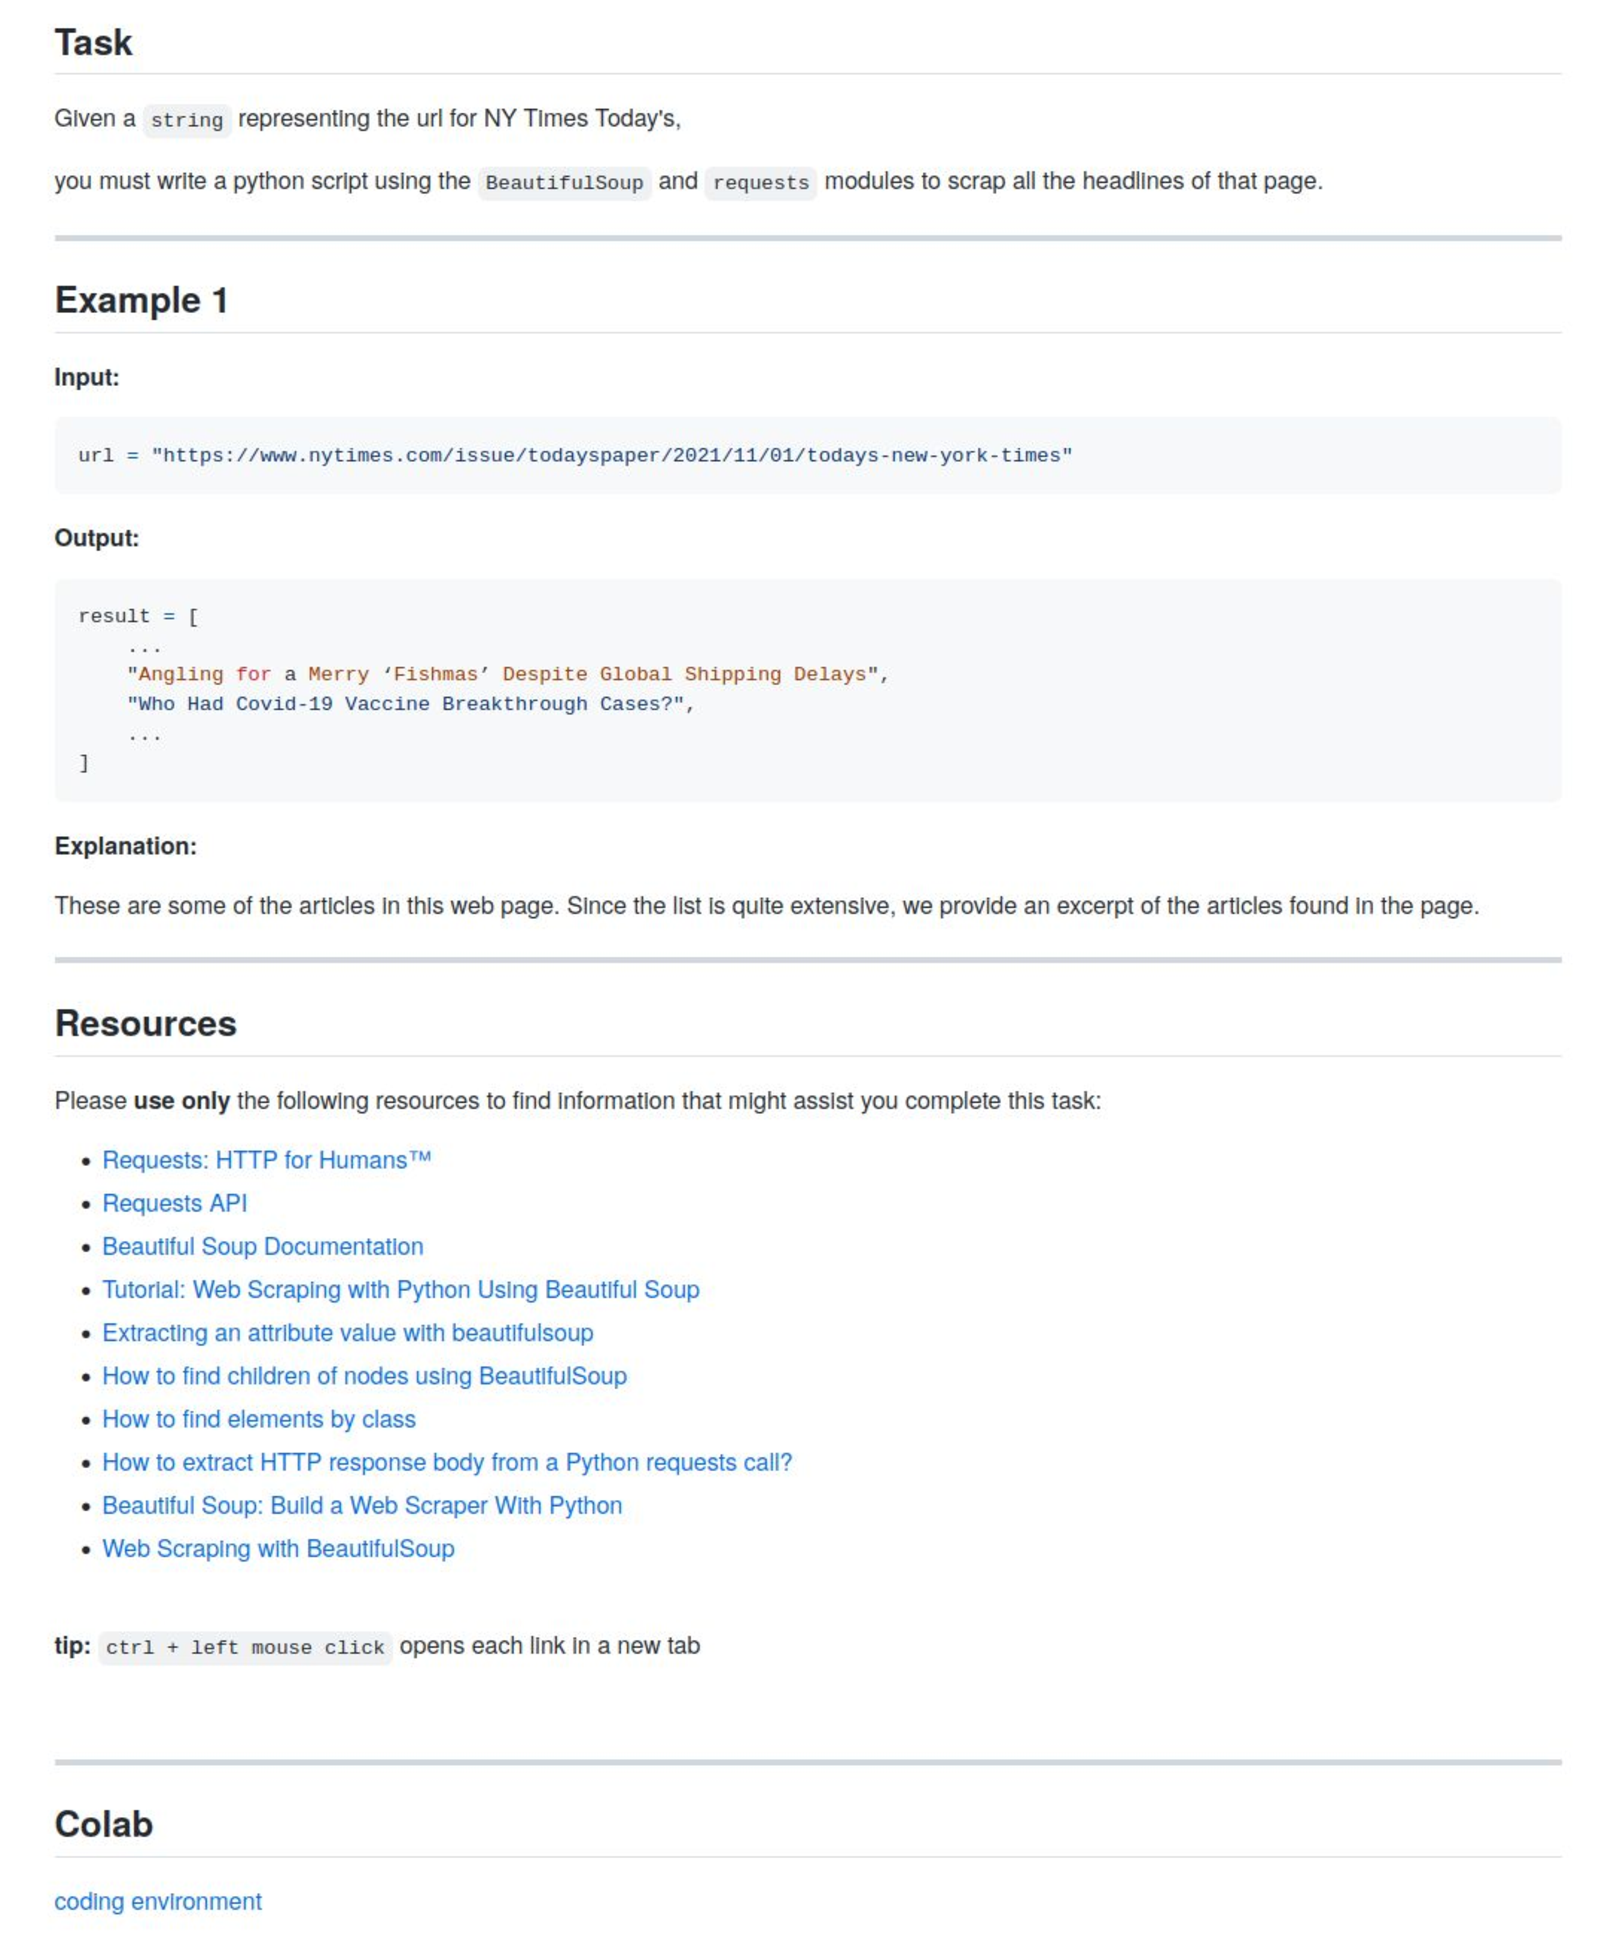
\includegraphics[width=1\textwidth]{cp6/task-github.pdf}
    \caption{Information shown in a task}
    \label{fig:nytimes-task-github}
\end{figure}



\clearpage

\begin{figure}
    \centering
    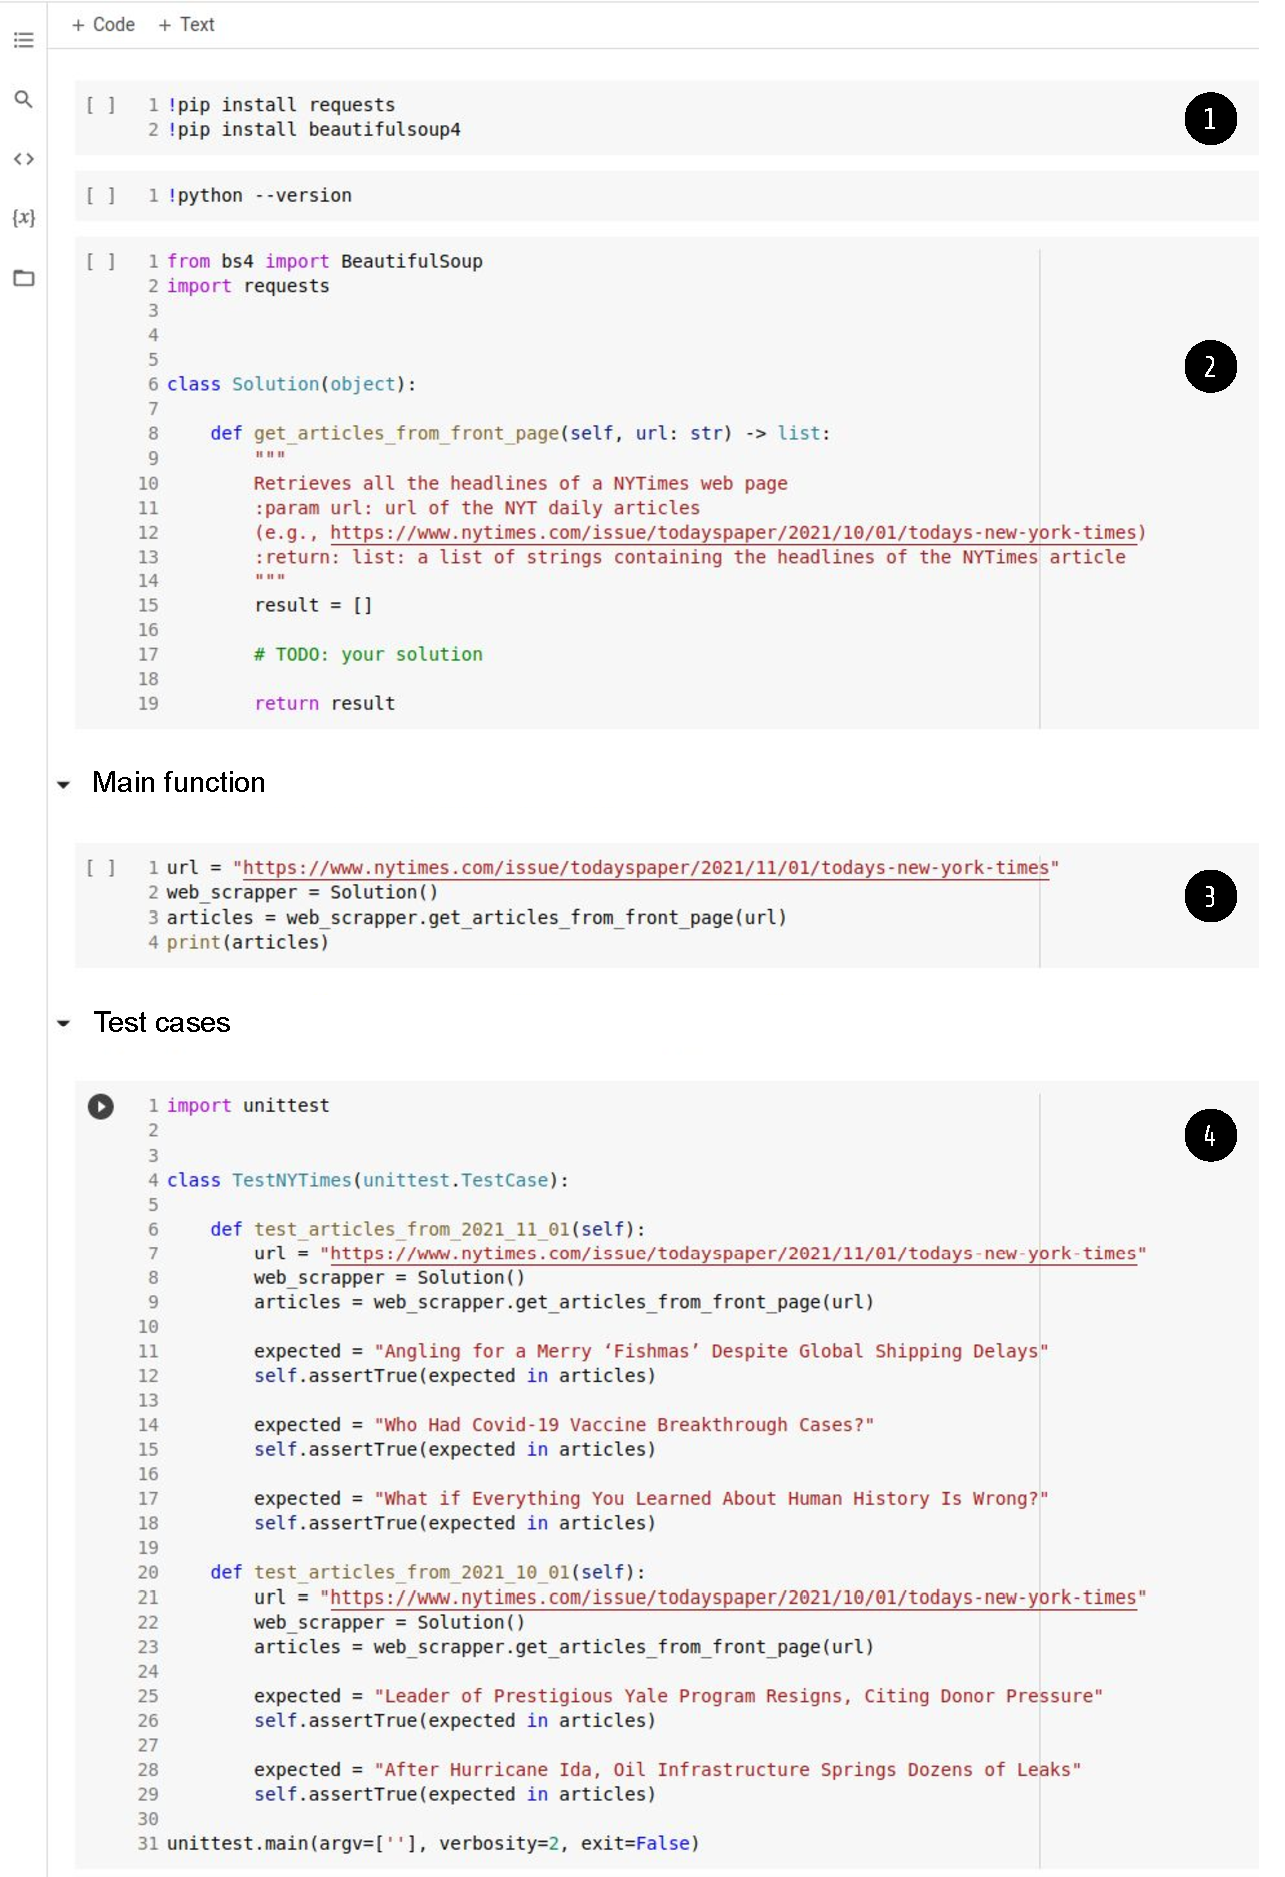
\includegraphics[width=\textwidth]{cp6/task-colab.pdf}
    \caption{Colab environment}
    \label{fig:nytimes-task-colab}
\end{figure}



\clearpage



\subsection{Participants}
\label{cp6:participants}


We advertised our study to professionals developers and to computer science students at  several universities. 
Our target population comprised professionals and third, fourth-year or graduate students.
We expected participants to have experience in Object-Oriented programming languages, and to consult API documentation when performing a programming task.
We gathered this background information as part of our demographics (Figure~\ref{fig:experiment-demographics})
and no participants were excluded
based on their background.

% \gcm{gender info?}



% (3 identified as female and 21 as male)


We obtained twenty four responses to our study advertisement (3 self-identified as female and 21 as male). 
At the time of the experiment, 10 participants were working as software
developers and 14 were students (11 graduate and 3 undergrad).
The majority of the students (71\%) also reported having some previous professional experience.


On average, participants self-reported 8 years of programming experience ({\small $\pm$} 3.8, ranging from 3 to 17 years).
The majority of the participants (54\%) had between 5 to 10 years of experience in Object-Oriented programming languages,
closely followed by participants  with  3 to 4 years of experience (29\%). 
Most of the participants also indicated that they did check API documents almost every time they performed a programming task. 


\begin{figure}
\begin{mdframed}[backgroundcolor=gray!15] 
\begin{scriptsize}

\noindent To witch gender do you identify? 

\medskip

\noindent If you are a student, in which year of the program are you at?  \smallskip

\quad $\square$~$1st$  
\quad $\square$~$2nd$  
\quad $\square$~$3rd$  
\quad $\square$~$4th$  
\quad $\square$~$5th+$ year 
\quad $\square$~\textit{graduate student} 

\medskip

\noindent For how many years have you been developing software?  

\medskip

\noindent For how many years have you been developing software \underline{professionaly}? 

\medskip

\noindent How many years of experience do you have in Object-Oriented programming languages?~\footnote{\scriptsize closed or open intervals notation} \smallskip

\quad $\square$~\textit{no experience} 
\quad $\square$ $(\infty, 1)$
\quad $\square$ $[1, 3)$
\quad $\square$ $[3, 5)$
\quad $\square$ $[5, 10)$
\quad $\square$ $[10, \infty)$

\medskip

\noindent With which frequency do you consult API documentation when performing a programming task?  \smallskip

\quad \textit{(never)} ~$1$ - $2$ - $3$ - $4$ - $5$ ~ ~\textit{(always)} 

\end{scriptsize}
\end{mdframed}
\caption{Background questions asked to a participant}
\label{fig:experiment-demographics}
\end{figure}

    






\subsection{Procedures}
\label{cp6:procedures}




The entry point to our experiment was our advertisement email.
The email disclosed the purpose of the experiment, eligibility criteria, an estimate of the time it would take to complete it as well as a link 
to a web survey containing the experiment's consent form and tasks. 


Once a participant consented to participate, the survey gathered demographics and then, 
it gave participants further instructions 
about how to perform each task, requesting them to install the our tool, a web browser plug-in.
Setup was followed by a short practice task---separate from the experimental tasks---that allowed participants to familiarize themselves with the content of a task, the tool, and the coding environment that we used (Colab). 


Once a participant completed the practice task, the survey randomly assigned to them a \textit{control} task, which was followed by a randomly assigned \textit{tool-assisted} tasks---different from the control task.
For each task, including the practice tasks, the survey provided to the participants a link 
to the task description (Figure~\ref{fig:nytimes-task-github}) and asked them to submit a solution for the task, i.e., written Python code. Table~\ref{tbl:python-task-distribution} shows the participants who performed each task in the control and tool-assisted groups. While tasks were randomly assigned, we made sure that an even number of participants attempted a task with and without tool support.


Once a participant submitted their solutions, the survey
asked them about any additional feeback that they wished to share and 
offered them the opportunity to enter a raffle for one of two iPads 64 GB 
to compensate them for their time, what concluded the experiment.






\begin{table}[h!]
\centering
\caption{List of participants who performed each task}
\begin{footnotesize}
\rowcolors{2}{}{lightgray}
\begin{tabular}{lllc}
\hline
\textbf{Task} & \textbf{Configuration} & \textbf{Participants who attempted the task} & \textbf{\#}                                                                              \\
\hline
\hline
%
%
\parbox[l][0.5cm][c]{1cm}{Distances}
& \textit{control group}        & $P3, P4, P8, P12, P16, P17,  P21, P22$  & 8 \\
\parbox[l][0.5cm][c]{1cm}{}
& \textit{with tool support}    & $P1, P5, P9, P13, P15, P18, P20, P23, P24$ & 9 \\
\hline
%
%
\parbox[l][0.5cm][c]{1cm}{NYTimes}
& \textit{control group}     & $P1, P2, P6, P10, P11, P14, P15, P20$ & 8 \\
\parbox[l][0.5cm][c]{1cm}{}
& \textit{with tool support} & $P3, P7, P12, P16, P17, P19, P21,  P22$ & 8 \\
\hline
%
%
\parbox[l][0.5cm][c]{1cm}{Titanic}       
& \textit{control group}     & $P5, P7, P9, P13, P18, P19, P23, P24$ & 8 \\
\parbox[l][0.5cm][c]{1cm}{}
& \textit{with tool support} & $P2, P4, P6, P8, P10, P11,  P14$ & 7 \\
\hline
%
%
\end{tabular}
\end{footnotesize}
\smallskip
\label{tbl:python-task-distribution}
\end{table}

    






\clearpage


\subsubsection{Control Task}
\label{cp6:procedures-manual}

% \gcm{Did they do this highlighting before the task or after? Confusing
% to say 'study tool' - just say you asked them to highlight sentences.
% 'study tool' makes it sound like the tool being studied, i.e., the
% one automaticalyl identifying text.}

In the \textit{control} task, we use the tool to gather text that a participant deems useful for the task at hand. In this task, 
the survey asked participants to use our tool to highlight sentences that they deemed useful and that provided information that assisted task completion---instructions similar to the ones used for the creation of the \acs{DS-android} corpus (Chapter~\ref{ch:android-corpus}). Participants could highlight text any time before submitting their solution. 
Based on observations from the pilots, the most common strategy we noticed was that of highlighting 
text on-the-fly, i.e., as a participant performed the task and consulted its artifacts, they would highlight text 
when reading each document.



Figure~\ref{fig:artifact-pre-highlight}
gives insight into how participants highlighted sentences. 
Whenever a participant inspected one of the artifacts available for their task, 
they could click on the \texttt{highlight} button in the tool's context menu.  
This would then instrumented the HTML of the page identifying individual sentences. 
A participant could hover over identified sentences and select them as relevant by clicking on the hovered text.
Once a participant had finished selecting sentences, they could submit 
their data also through the tool's context menu.


% As an example, Figure~\ref{fig:artifact-pre-highlight} shows a sentence discussing the \texttt{find\_all} method, which 
% one of the participants in our experiment deemed 
% relevant to the \texttt{NYTimes} task.
% Based on the pilots, we observed that the most natural flow adopted by participants was to highlight text on-the-fly. That is, they indicated what text 
% was relevant for the task at hand while they consulted each artifact and wrote their solution. 



\begin{figure}
    \centering
    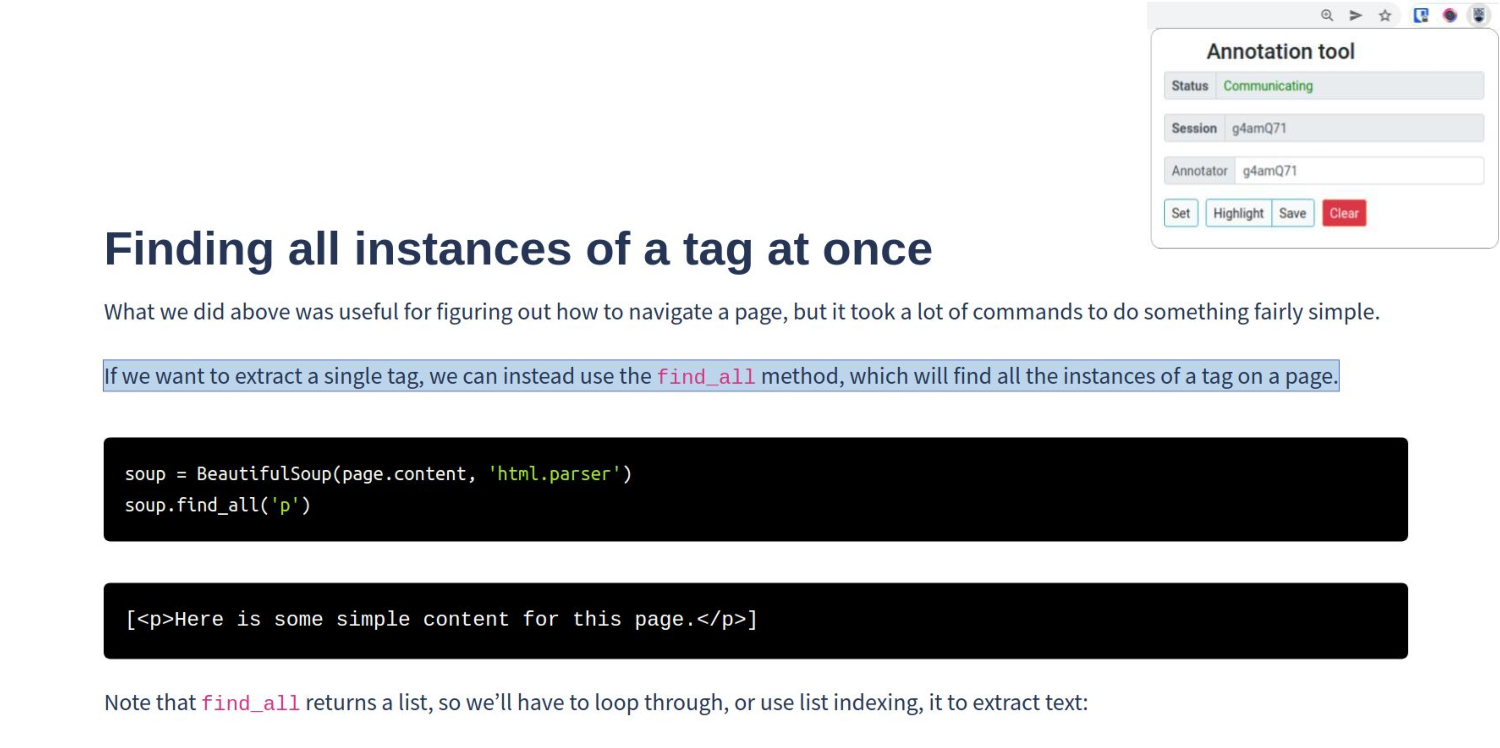
\includegraphics[width=1.0\textwidth]{cp6/manual-task.pdf}
    \caption{Study's tool context menu (top-right corner) and a sentence highlighted by a participant}
    \label{fig:artifact-pre-highlight}
\end{figure}




\subsubsection{Tool-assisted Task}
\label{cp6:procedures-tool-assisted}


In the tool-assisted task, our tool automatically highlighted text that 
its underlying semantic-based technique identified as relevant to the participant's task\footnote{
    We configure the tool to identify no more than 10\% of the sentences of an input artifact as relevant.
    This number was determined based on the average number of sentences indicated as relevant by human annotators in the artifacts of the \acs{DS-android} corpus.
}.
The highlights were shown in a format similar to the one in Figure~\ref{fig:artifact-pre-highlight}, but without the need for any actions by a participant.




For this task, when a participant submitted their solution, we asked them to 
rate on a 5 points Likert scale~\cite{likert1932technique} how helpful were the highlights shown by the tool.
Figure~\ref{fig:experiment-rating} shows an example of how we gathered data about the usefulness of the text automatically identified.
Participants rated highlights on a per artifact basis.
We gather input at the artifact level because it would be too demanding for a participant 
to provide individual feedback on each of the highlights shown
in the time that we estimated and that we advertised for the study.
Section~\ref{cp6:threats} discusses  threats that arise from this decision.




\begin{figure}
\begin{mdframed}[backgroundcolor=gray!15] 
\begin{scriptsize}

\noindent \textbf{1.} Indicate whether you agree with the following statement:

\medskip

\quad \textit{The highlights in \textcolor{steelblue}{``How to extract HTTP response body from a Python requests call''} were helpful to} 

\quad \textit{correctly accomplish the task in question.}  \smallskip

\smallskip

\quad \quad \textit{(Strongly disagree)} ~$1$ - $2$ - $3$ - $4$ - $5$ ~\textit{(Strongly agree)} 


\bigskip


\noindent \textbf{2.} Indicate whether you agree with the following statement:

\medskip

\quad \textit{The highlights in \textcolor{steelblue}{``BeautifulSoup tutorial: Scraping web pages with Python''} were helpful to} 

\quad \textit{correctly accomplish the task in question.}  \smallskip

\smallskip

\quad \quad \textit{(Strongly disagree)} ~$1$ - $2$ - $3$ - $4$ - $5$ ~\textit{(Strongly agree)} 

\centering 

...

\end{scriptsize}
\end{mdframed}
\caption{Questions asking a participant to rate the usefulness of the highlights shown in two artifacts; by clicking on the name of an artifact, a participant could revisit the highlights of that artifact}
\label{fig:experiment-rating}
\end{figure}

    



\subsection{Summary of experimental procedures}


We have described experimental procedures 
where participants attempted two programming tasks each.
These procedures allowed us to gather:


\begin{enumerate}
\item a participant's submitted solution (written Python code) for each task;
\item text that participants deemed relevant in the artifacts of the control task;
\item the usefulness of the highlights shown in a tool-assisted task; and
\item any additional feedback (written text) that a participant wished to provide.
\end{enumerate}


We use this data to investigate whether 
a tool embedding a semantic-based technique helps developers complete a software task. 


% \clearpage


